%UNIT 16: Introduction to Laplace Transforms
%%%%%%%%%%%%%%%%%%%%%%%%%%%
%%%% Put the following at the top of each .tex file  %
\pagestyle{fancy}
\renewcommand{\theUnit}{6.2}
\ifthenelse{\isundefined{\UnitPageNumbers}}{}{\setcounter{page}{1}}
\rhead{Section \theUnit: Solving ODE's with Laplace Transform}
\lhead{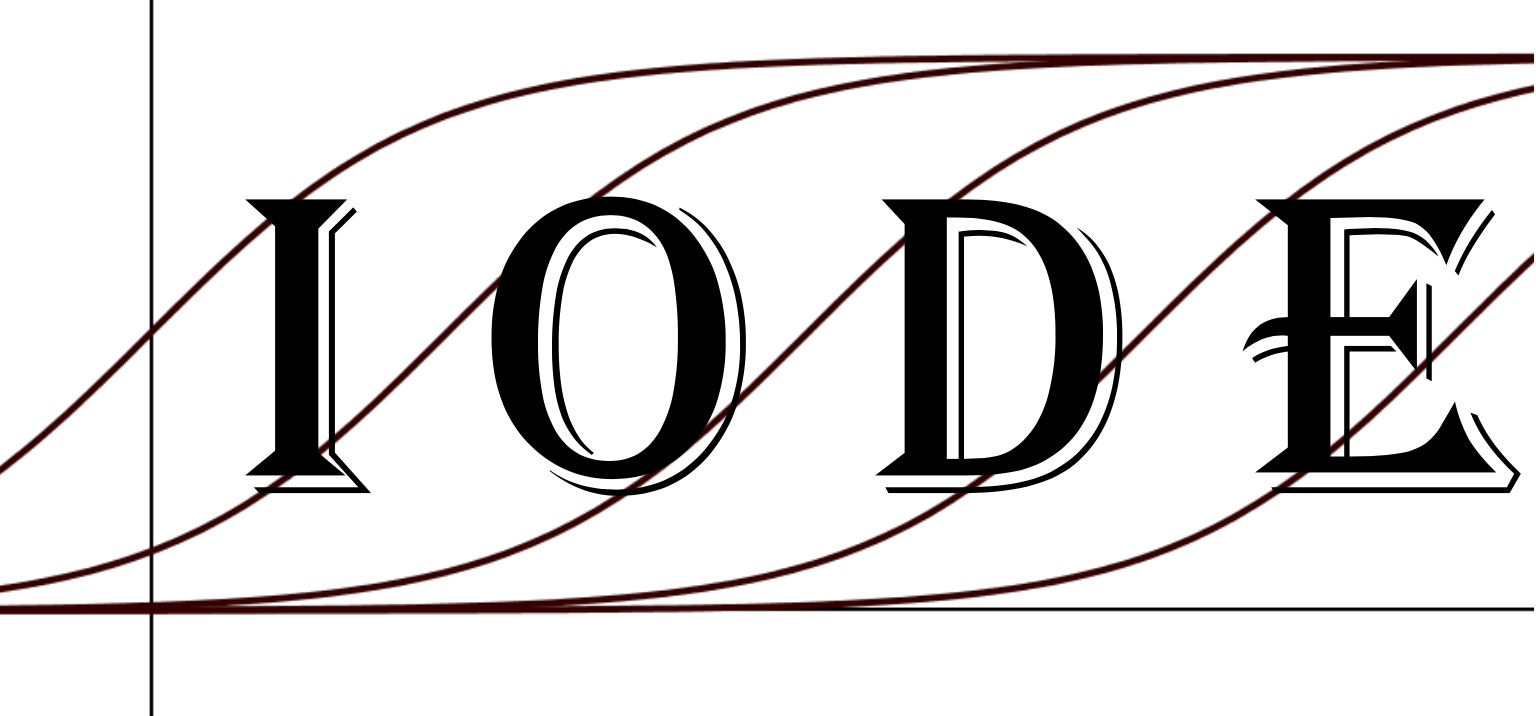
\includegraphics[width=1.25cm]{IODE-logo.png}}
\rfoot{\mypage}
\lfoot{}
\cfoot{}
\fancypagestyle{firstfooter}{\footskip = 50pt}
\renewcommand{\footrulewidth}{.4pt}
%%%%%%%%%%%%%%%%%%%%%%%%%%%
\vspace*{-20pt} \thispagestyle{firstfooter}

\pagebegin{Common Laplace Transforms and Properties}

\begin{center}
\begin{tabular}{|l|l|}
\hline
$f(t)$ & $F(s) = \Lap \left\{ f(t) \right\}$ \\
\hline
$1$ & $\dsty \frac{1}{s}, \ s > 0$\\
\hline
$e^{at}$ & $\dsty \frac{1}{s-a}, \ s > a$\\
\hline
$t^n, \ n=1,2, \ldots$ & $\dsty \frac{n!}{s^{n+1}}, \ s > 0$\\
\hline
$\sin{(bt)}$ & $\dsty \frac{b}{s^2+b^2}, \ s > 0$\\
\hline
$\cos{(bt)}$ & $\dsty \frac{s}{s^2+b^2}, \ s > 0$\\
\hline
$e^{at}t^n, \ n=1,2, \ldots$ & $\dsty \frac{n!}{(s-a)^{n+1}}, \ s > a$\\
\hline
$e^{at}\sin{(bt)}$ & $\dsty \frac{b}{(s-a)^2+b^2}, \ s > a$\\
\hline
$e^{at}\cos{(bt)}$ & $\dsty \frac{s-a}{(s-a)^2+b^2}, \ s > a$\\
\hline
\end{tabular}
\end{center}

 \textbf{Properties:}


\begin{enumerate}[label=L.\arabic*]
\ii $\mathscr{L} \left\{ cf(t) \right\} = c  \mathscr{L} \left\{ f(t) \right\}$, where $c$ is a constant. \ms

\ii $\mathscr{L} \left\{ f_1(t) + f_2(t) \right\} = \mathscr{L} \left\{ f_1(t) \right\} + \mathscr{L} \left\{ f_2(t)\right\}$ \ms

\ii If $F(s) = \mathscr{L} \left\{ f(t) \right\}$ exists for all $s > \alpha$, then $\dsty \mathscr{L} \left\{ e^{at} f(t) \right\} = F(s-a)$ for all $s>\alpha + a$.  \ms

\ii If $F(s) =\mathscr{L} \left\{ f(t) \right\}$ exists for all $s > \alpha$, then for all $s>\alpha$,
\[ \mathscr{L} \left\{ f^{(n)}(t) \right\} = s^n  \mathscr{L}  \{ f(t) \}-s^{n-1} f(0)- s^{n-2} f'(0) - \ldots - f^{(n-1)}(0).\] \ms

%\ii If $F(s) =\mathscr{L} \left\{ f(t) \right\}$ exists for all $s > \alpha$, then $\dsty \mathscr{L} \left\{ f'(t) \right\} = sF(s) -f(0)$ for all $s > \alpha$.
%\ii If $F(s) =\mathscr{L} \left\{ f(t) \right\}$ exists for all $s > \alpha$, then $\dsty \mathscr{L} \left\{ f''(t) \right\} = s^2 F(s) - sf(0)- f'(0)$ for all $s > \alpha$.

\ii If $F(s) =\mathscr{L} \left\{ f(t) \right\}$ exists for all $s > \alpha$, then $\dsty \mathscr{L} \left\{ t^n f(t) \right\} = (-1)^n \frac{d^nF}{ds^n}$ for all $s > \alpha$.
\ee

%\bb
%\ii $\mathscr{L} \left\{ cf(t) \right\} = c  \mathscr{L} \left\{ f(t) \right\}$, where $c$ is a constant.
%\ii $\mathscr{L} \left\{ f_1(t) + f_2(t) \right\} = \mathscr{L} \left\{ f_1(t) \right\} + \mathscr{L} \left\{ f_2(t)\right\}%$
%\ii If $F(s) = \mathscr{L} \left\{ f(t) \right\}$ exists for all $s > \alpha$, then $\dsty \mathscr{L} \left\{ e^{at} f(t) \right\} = F(s-a)$ for all $s>\alpha + a$. 
%\ii If $F(s) =\mathscr{L} \left\{ f(t) \right\}$ exists for all $s > \alpha$, then for all $s>\alpha$:
%\bi
%\ii $\dsty \mathscr{L} \left\{ f'(t) \right\} = sF(s) -f(0)$ for all $s > \alpha$, and thus
%\ii $\dsty \mathscr{L} \left\{ f^{(n)}(t) \right\} = s^n\mathscr{L} \{ f(t) \}-s^{n-1} f(0)- s^{n-2} f'(0) - \ldots - f^{(n-1)}(0).$
%\ei
%\ii If $F(s) =\mathscr{L} \left\{ f(t) \right\}$ exists for all $s > \alpha$, then $\dsty \mathscr{L} \left\{ t^n f(t) \right\} = (-1)^n \frac{d^nF}{ds^n}$ for all $s > \alpha$.
%\ee

\clearpage

\pagebegin{Section 6.2: Solving ODE's}


\bb[label=Step \arabic*]
\ii Take the Laplace transform of both sides. Refer to properties.
\ii Rearrange and group like terms to solve for $\mathcal{L}\{y(t)\}=Y(s)$
\ii Take the inverse Laplace transform and solve for $y(t) = \mathcal{L}^{-1}\{Y(x) \}$.
\ee

\ms

\hline

\ms

\bb
\ii Solve the initial value problem using Laplace Transforms (not previous methods).  \label{17problem6}

\bb
\ii $y''-2y'+5y=0$ with $y(0)=2$ and $y'(0)=4$. \label{17problem6a}
\vfill
\clearpage
\ii $y''-y'-2y=0$ with $y(0)=-2$ and $y'(0)=5$. \label{17problem6b} %Q2
\vfill
\ii $y''-4y'-5y=4e^{3t}$ with $y(0)=2$ and $y'(0)=7$. \label{17problem6c} %Q6
\vfill
\clearpage
\ii $ty''-ty'+y=2$ with $y(0)=2$ and $y'(0)=-1$. \label{17problem6d}
\vfill
\clearpage
\ii $y''+ty'-y=0$ with $y(0)=0$ and $y'(0)=3$. \label{17problem6e}
\vfill
\ee
\ee
